%%%%%%%%%%%%%%%%%%%%%%%%%%%%%%%%%%%%%%%%%
% Beamer Presentation
% LaTeX Template
% Version 1.0 (10/11/12)
%
% This template has been downloaded from:
% http://www.LaTeXTemplates.com
%
% License:
% CC BY-NC-SA 3.0 (http://creativecommons.org/licenses/by-nc-sa/3.0/)
%
%%%%%%%%%%%%%%%%%%%%%%%%%%%%%%%%%%%%%%%%%

%----------------------------------------------------------------------------------------
%	PACKAGES AND THEMES
%----------------------------------------------------------------------------------------

\documentclass[handout]{beamer}

\mode<presentation> {

% The Beamer class comes with a number of default slide themes
% which change the colors and layouts of slides. Below this is a list
% of all the themes, uncomment each in turn to see what they look like.

%\usetheme{default}
%\usetheme{AnnArbor}
%\usetheme{Antibes}
%\usetheme{Bergen}
%\usetheme{Berkeley}
%\usetheme{Berlin}
%\usetheme{Boadilla}
%\usetheme{CambridgeUS}
%\usetheme{Copenhagen}
%\usetheme{Darmstadt}
%\usetheme{Dresden}
%\usetheme{Frankfurt}
%\usetheme{Goettingen}
%\usetheme{Hannover}
%\usetheme{Ilmenau}
%\usetheme{JuanLesPins}
%\usetheme{Luebeck}
\usetheme{Madrid}
%\usetheme{Malmoe}
%\usetheme{Marburg}
%\usetheme{Montpellier}
%\usetheme{PaloAlto}
%\usetheme{Pittsburgh}
%\usetheme{Rochester}
%\usetheme{Singapore}
%\usetheme{Szeged}
%\usetheme{Warsaw}

% As well as themes, the Beamer class has a number of color themes
% for any slide theme. Uncomment each of these in turn to see how it
% changes the colors of your current slide theme.

%\usecolortheme{albatross}
%\usecolortheme{beaver}
%\usecolortheme{beetle}
%\usecolortheme{crane}
%\usecolortheme{dolphin}
%\usecolortheme{dove}
%\usecolortheme{fly}
%\usecolortheme{lily}
%\usecolortheme{orchid}
%\usecolortheme{rose}
%\usecolortheme{seagull}
%\usecolortheme{seahorse}
%\usecolortheme{whale}
%\usecolortheme{wolverine}

%\setbeamertemplate{footline} % To remove the footer line in all slides uncomment this line
%\setbeamertemplate{footline}[page number] % To replace the footer line in all slides with a simple slide count uncomment this line

%\setbeamertemplate{navigation symbols}{} % To remove the navigation symbols from the bottom of all slides uncomment this line
}

\usepackage{graphicx} % Allows including images
\usepackage{booktabs} % Allows the use of \toprule, \midrule and \bottomrule in tables
\usepackage{cool}
\usepackage{tikz}
\usepackage{amsmath}
\usepackage{xcolor}
\usepackage{hyperref}

\DeclareMathOperator*{\argmax}{argmax}
\DeclareMathOperator*{\argmin}{argmin}
\usetikzlibrary{positioning}

%----------------------------------------------------------------------------------------
%	TITLE PAGE
%----------------------------------------------------------------------------------------

\title[RL for Finance]{CME 241: Reinforcement Learning for Stochastic Control Problems in Finance} % The short title appears at the bottom of every slide, the full title is only on the title page

\author{Ashwin Rao} % Your name
\institute[Stanford] % Your institution as it will appear on the bottom of every slide, may be shorthand to save space
{ICME, Stanford University
 % Your institution for the title page
}

\date{} % Date, can be changed to a custom date

\begin{document}
\begin{frame}
\titlepage % Print the title page as the first slide
\end{frame}

% \begin{frame}
% \frametitle{Overview} % Table of contents slide, comment this block out to remove it
% \tableofcontents % Throughout your presentation, if you choose to use \section{} and \subsection{} commands, these will automatically be printed on this slide as an overview of your presentation
% \end{frame}

\begin{frame}
\frametitle{Meet your Instructor}
\pause
\begin{itemize}[<+->]
\item My educational background: Algorithms Theory \& Abstract Algebra
\item 10 years at Goldman Sachs (NY) {\em Rates/Mortgage Derivatives} Trading
\item 4 years at Morgan Stanley as {\em Managing Director - Market Modeling}
\item Founded Tech Startup {\em ZLemma}, Acquired by hired.com in 2015
\item One of our products was algorithmic jobs/career guidance for students
\item I've been teaching short/medium-length courses for 25 years
\item Topics across Pure \& Applied Math, CS, Programming, Finance
\item Current Interest: A.I. for Dynamic Decisioning under Uncertainty
\item V.P. Data Science at Target focused on Optimal Inventory Control
\item Joined Stanford ICME as Adjunct in Fall 2018
\item Apart from CME 241, I am a technical mentor to ICME students
\end{itemize}
\end{frame}


\begin{frame}
\frametitle{Requirements and Setup}
\pause
\begin{itemize}[<+->]
\item (Light) Pre-requisites:
\begin{itemize}
\item Undergraduate-level background in Applied Mathematics (Linear Algebra, Probability Theory, Optimization)
\item Background in Data Structures \& Algorithms, with programming experience in numpy/scipy
\item Basic background in Pricing and Portfolio Theory, but we will do an overview of the requisite Finance/Economics
\item No background required in MDP, DP, RL (we will cover these topics from scratch)
\end{itemize}
\item Install Python 3 and supporting editor/IDE (eg: PyCharm)
\item Create git repo for this course (for assignments/sharing)
\item Send the git repo details to the Course Assistant (for reviews/grading)
\item Install LaTeX and supporting editor (eg: TeXShop)
\end{itemize}
\end{frame}


\begin{frame}
\frametitle{Housekeeping}
\pause
\begin{itemize}[<+->]
\item Grade based on:
\begin{itemize}
\item 25\%: Mid-Term Exam
\item 35\%: Final Exam
\item 30\%: Programming and Technical Writing Assignments
\item 10\%: Class Participation
\end{itemize} 
\item Passing grade fetches 3 credits, can be applied towards MCF degree
\item Wed and Fri 4:30pm - 5:50pm, 01/07/2019 - 03/15/2019
\item Classes in \href{https://campus-map.stanford.edu/?srch=200-203}{\underline{\textcolor{blue}{Building 200 (Lane History Corner) - Room 203}}}
\item Appointments: Any time Fridays or an hour before class Wednesdays
\item Use appointments time to discuss theory as well as your code
\item Course Web Site: \href{cme241.stanford.edu}{\underline{\textcolor{blue}{cme241.stanford.edu}}}
\item Course Assistant (CA) is Jeffrey Gu (ICME student)
\item My e-mail: \href{mailto:ashwin.rao@stanford.edu}{\underline{\textcolor{blue}{ashwin.rao@stanford.edu}}}, CA e-mail: \href{mailto:jeffgu@stanford.edu}{\underline{\textcolor{blue}{jeffgu@stanford.edu}}}
\end{itemize}
\end{frame}

\begin{frame}
\frametitle{Resources}
\pause
\begin{itemize}[<+->]
\item I recommend \href{http://incompleteideas.net/book/the-book-2nd.html}{\underline{\textcolor{blue}{Sutton-Barto}}} as the companion book for this course
\begin{itemize}
\item I won't follow the structure of Sutton-Barto book
\item But I will follow his approach/treatment
\end{itemize}
\item I will follow the structure of \href{http://www0.cs.ucl.ac.uk/staff/d.silver/web/Teaching.html}{\underline{\textcolor{blue}{David Silver's RL course}}}
\begin{itemize}
\item I encourage you to augment my lectures with David's lecture videos
\item Occasionally, I will wear away or speed up/slow down from this flow
\end{itemize}
\item We will do a bit more Theory \& a lot more coding (relative to above)
\item You can freely use my \href{https://github.com/coverdrive/MDP-DP-RL}{\underline{\textcolor{blue}{open-source code}}} for your coding work
\begin{itemize}
\item I expect you to duplicate the functionality of above code in this course
\end{itemize}
\item We will go over some classical papers on the Finance applications
\item To understand in-depth the analytical solutions in simple settings
\item I will augment the above content with many of my own slides
\item All of this will be organized on the course web site
\end{itemize}
\end{frame}

\begin{frame}
\frametitle{Learning Tenets (to thrive in this course)}
\pause
\begin{itemize}[<+->]
\item When learning Theory, blend notational rigor with concepts intuition
\item LaTeX the mathematical formalism of lecture contents with precision
\item Programming is a powerful tool to grasp mathematical concepts
\item Code modularity/re-use is important (leverage OOP/FP paradigms)
\item Always start with a simple model/algorithm, evolve incrementally
\item Important to model various frictions encountered in real-world trading
\item Discuss the ideas you learn with others (incl. with the CA and me)
\item Remember this is an intro course. Avoid advanced RL at this stage
\item Success := {\bf Blending Theory, Algos/Code, Real-World Modeling}
\end{itemize}
\end{frame}

\begin{frame}
\frametitle{A.I. for Dynamic Decisioning under Uncertainty}
\pause
\begin{itemize}[<+->]
\item Let's browse some terms used to characterize this branch of A.I.
\item {\em Stochastic}: Uncertainty in key quantities, evolving over time
\item {\em Optimization}: A well-defined metric to be maximized (``The Goal'')
\item {\em Dynamic}:  Decisions need to a function of the changing situations
\item {\em Control}: Overpower uncertainty by persistent steering towards goal
\item Jargon overload due to confluence of Control Theory, O.R. and A.I.
\item For language clarity, let's just refer to this area as {\em Stochastic Control}
\item The core framework is called {\em Markov Decision Processes} (MDP)
\end{itemize}
\end{frame}



\begin{frame}
\frametitle{The MDP Framework}
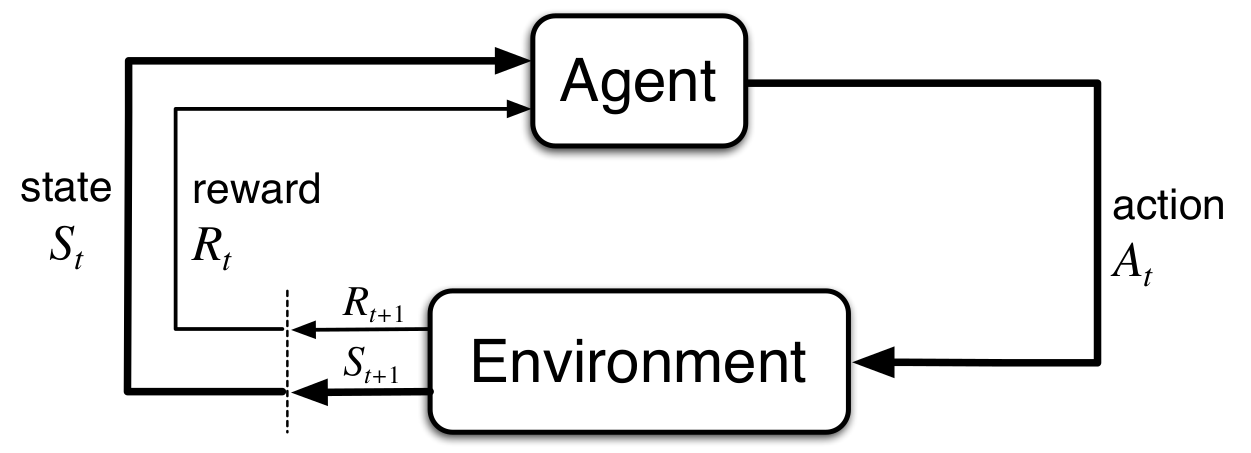
\includegraphics[width=12cm, height=7cm]{MDP.png}
\end{frame}

\begin{frame}
\frametitle{Components of the MDP Framework}
\pause
\begin{itemize}[<+->]
\item The {\em Agent} and the {\em Environment} interact in a time-sequenced loop
\item {\em Agent} responds to [{\em State}, {\em Reward}] by taking an {\em Action}
\item {\em Environment} responds by producing next step's (random) {\em State}
\item {\em Environment} also produces a (random) scalar denoted as {\em Reward}
\item Each {\em State} is assumed to have the {\em Markov Property}, meaning:
\begin{itemize}
\item Next {\em State/Reward} depends only on Current {\em State} (for a given {\em Action})
\item Current {\em State} captures all relevant information from {\em History}
\item Current {\em State} is a sufficient statistic of the future (for a given {\em Action})
\end{itemize} 
\item Goal of {\em Agent} is to maximize {\em Expected Sum} of all future {\em Reward}s
\item By controlling the ({\em Policy} : {\em State} $\rightarrow$ {\em Action}) function
\item This is a dynamic (time-sequenced control) system under uncertainty
\end{itemize}
\end{frame}

\begin{frame}
\frametitle{Formal MDP Framework}
\pause
The following notation is for discrete time steps. Continuous-time formulation is analogous (often involving
\href{https://github.com/coverdrive/technical-documents/blob/master/finance/cme241/StochasticCalculusFoundations.pdf}{\underline{\textcolor{blue}{Stochastic Calculus}}})
\begin{itemize}[<+->]
\item Time steps denoted as $t = 1, 2, 3, \ldots$
\item Markov States $S_t \in \mathcal{S}$ where $\mathcal{S}$ is the State Space
\item Actions $A_t \in \mathcal{A}$ where $\mathcal{A}$ is the Action Space
\item Rewards $R_t \in \mathbb{R}$ denoting numerical feedback\
\item Transitions $p(s',r|s,a) = Pr\{S_{t+1}=s',R_{t+1}=r|S_t=s,A_t=a\}$
\item $\gamma \in [0,1]$ is the Discount Factor for Reward when defining {\em Return}
\item Return $G_t = R_t + \gamma \cdot R_{t+1} + \gamma^2 \cdot R_{t+1} + \ldots$
\item Policy $\pi(a|s)$ is probability that Agent takes action $a$ in states $s$
\item The goal is find a policy that maximizes  $\mathbb{E}[G_t|S_t = s]$ for all $s \in \mathcal{S}$
\end{itemize}
\end{frame}

\begin{frame}
\frametitle{How a baby learns to walk}
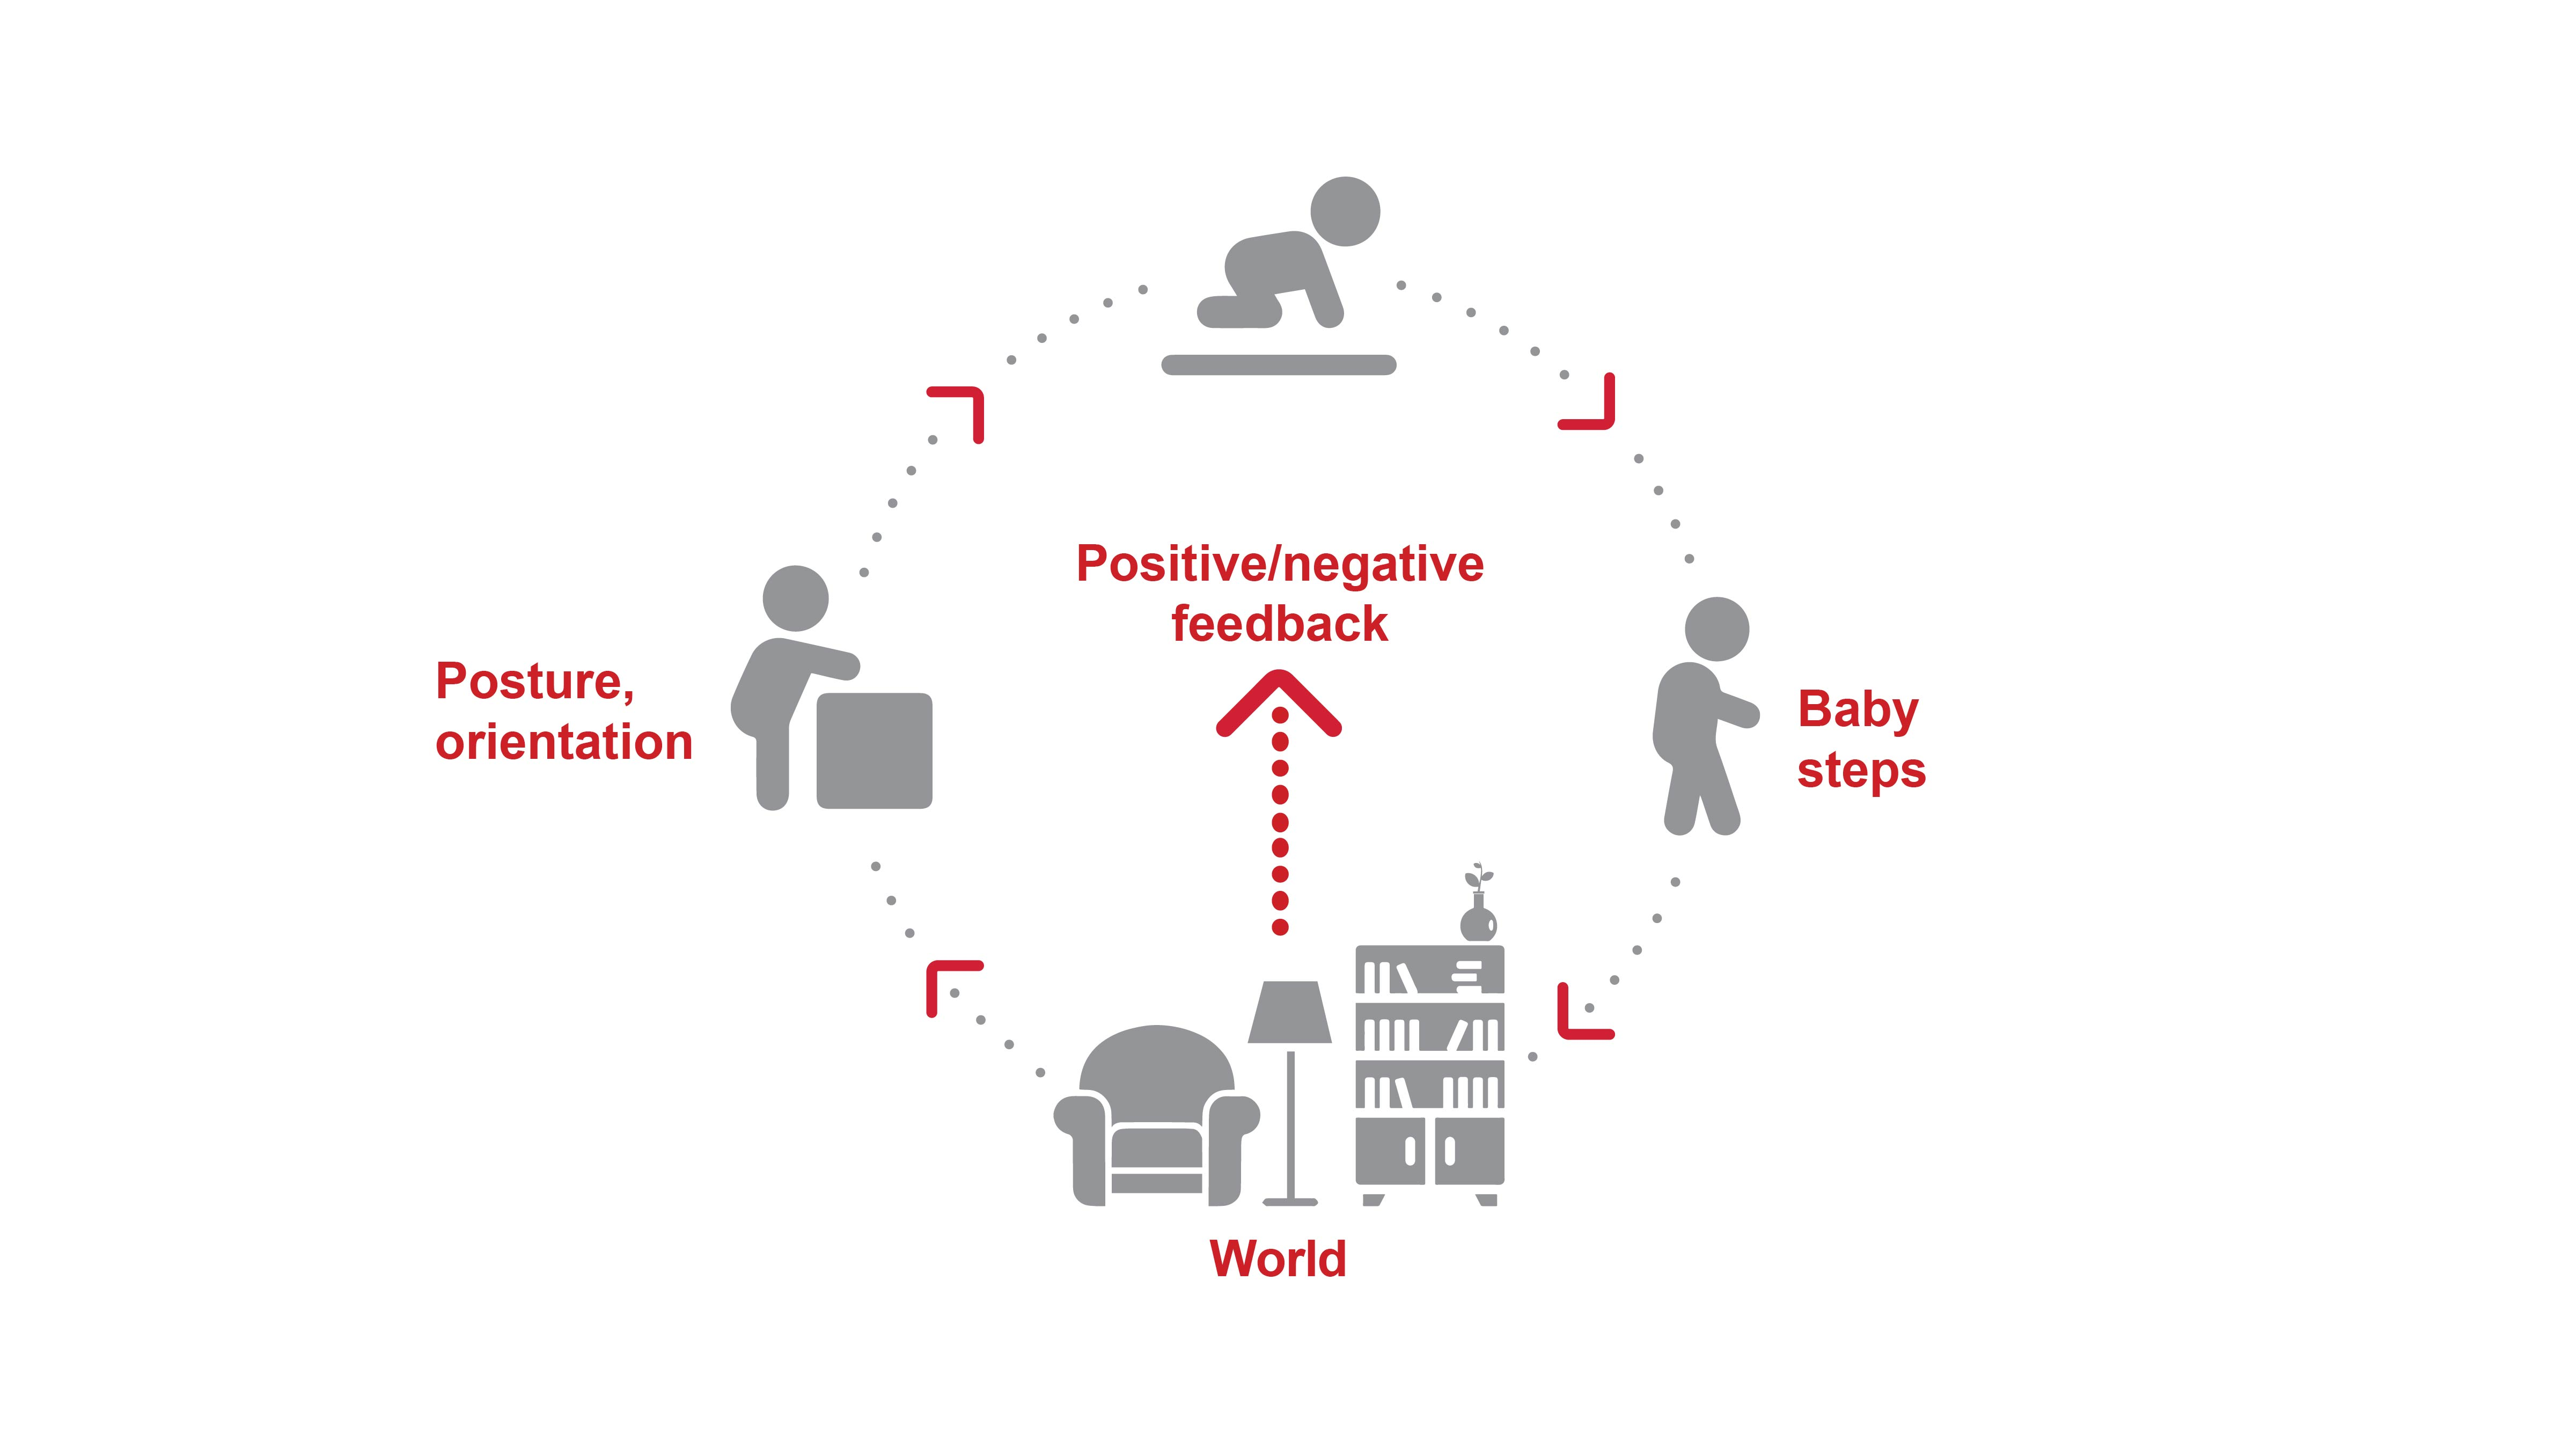
\includegraphics[width=13cm, height=8cm]{BabyMDP.jpg}
\end{frame}

\begin{frame}
\frametitle{Many real-world problems fit this MDP framework}
\pause
\begin{itemize}[<+->]
\item Self-driving vehicle (speed/steering to optimize safety/time)
\item Game of Chess (Boolean {\em Reward} at end of game)
\item Complex Logistical Operations (eg: movements in a Warehouse)
\item Make a humanoid robot walk/run on difficult terrains
\item Manage an investment portfolio
\item Control a power station
\item Optimal decisions during a football game
\item Strategy to win an election (high-complexity MDP)
\end{itemize}
\end{frame}

\begin{frame}
\frametitle{Self-Driving Vehicle}
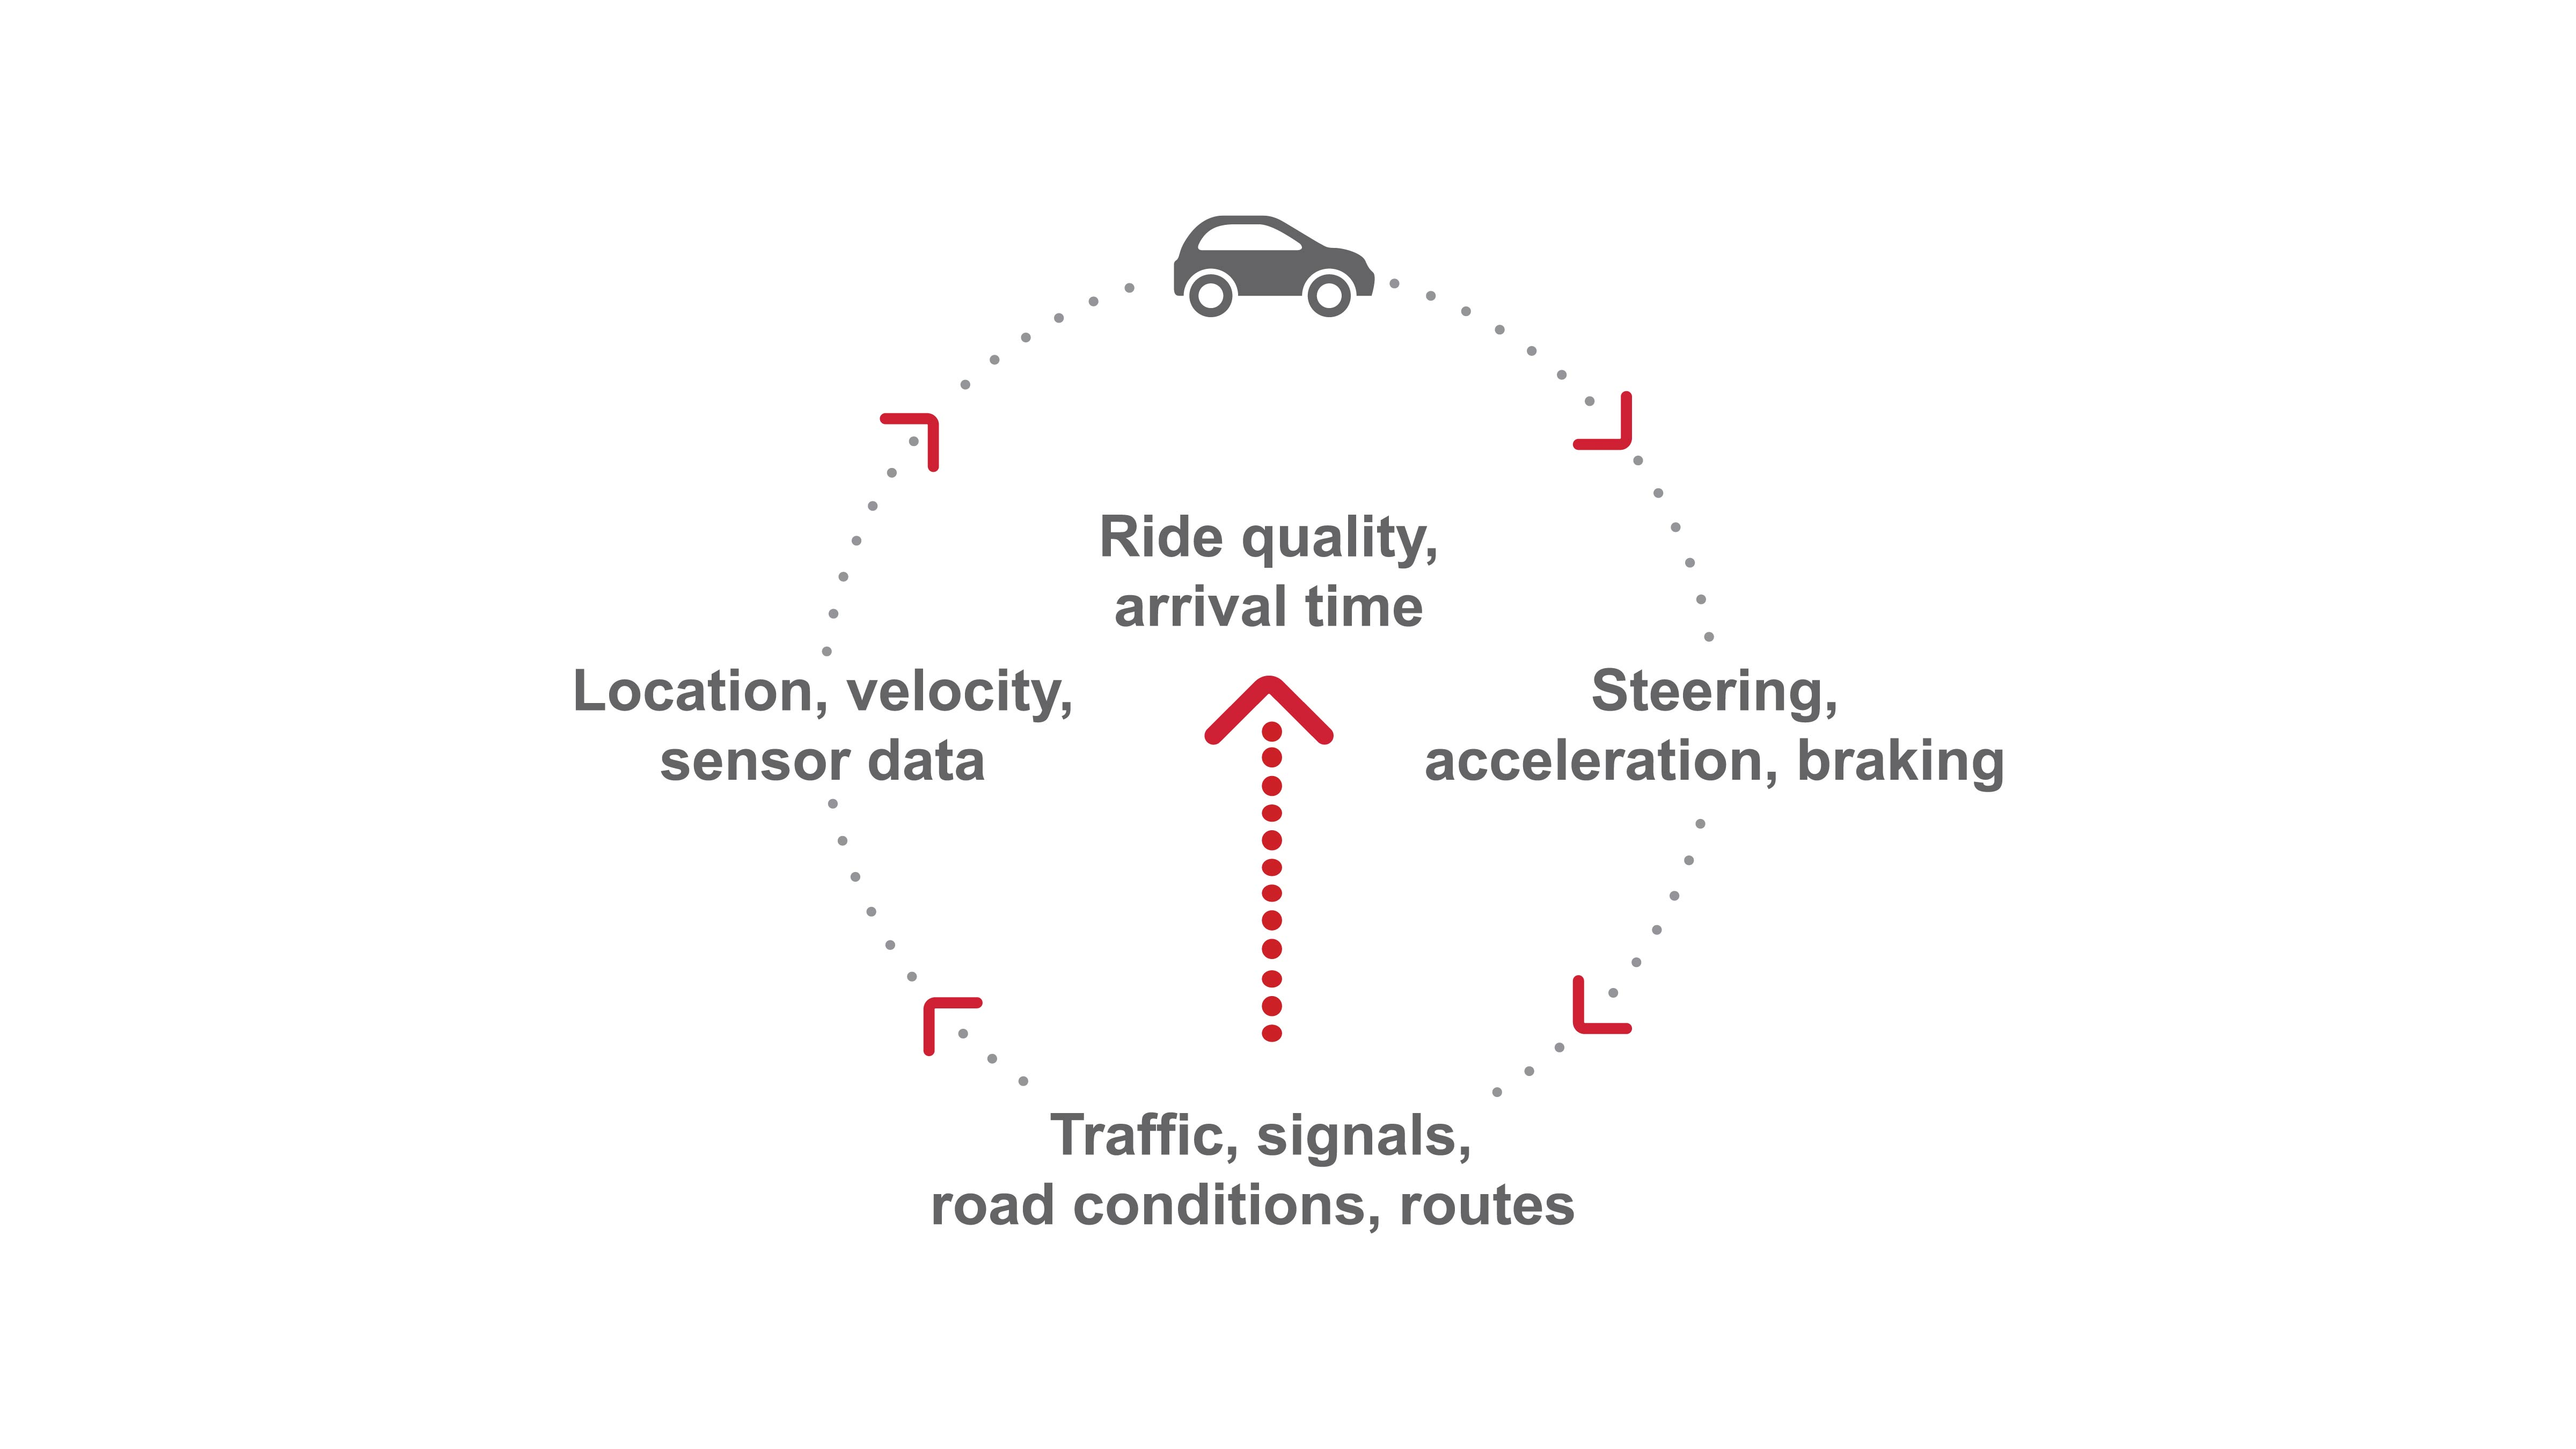
\includegraphics[width=13cm, height=8cm]{CarMDP.jpg}
\end{frame}

\begin{frame}
\frametitle{Why are these problems hard?}
\pause
\begin{itemize}[<+->]
\item {\em State} space can be large or complex (involving many variables)
\item Sometimes, {\em Action} space is also large or complex
\item No direct feedback on ``correct'' {\em Actions} (only feedback is {\em Reward})
\item Time-sequenced complexity ({\em Actions} influence future {\em States/Actions})
\item {\em Action}s can have delayed consequences (late {\em Reward}s)
\item {\em Agent} often doesn't know the {\em Model} of the {\em Environment}
\item ``Model'' refers to probabilities of state-transitions and rewards
\item So, {\em Agent} has to learn the {\em Model} AND solve for the Optimal {\em Policy}
\item {\em Agent} {\em Action}s need to tradeoff between ``explore'' and ``exploit''
\end{itemize}
\end{frame}

\begin{frame}
\frametitle{Value Function and Bellman Equations}
\pause
\begin{itemize}
\item Value function (under policy $\pi$) $V_{\pi}(s) = \mathbb{E}[G_t|S_t = s]$ for all $s \in \mathcal{S}$
\pause
$$V_{\pi}(s) = \sum_{a} \pi(a|s) \sum_{s',r} p(s',r|s,a) \cdot (r + \gamma V_{\pi}(s')) \mbox{ for all } s \in \mathcal{S}$$
\pause
\item Optimal Value Function $V_{*}(s) = \max_{\pi} V_{\pi}(s) \mbox{ for all } s \in \mathcal{S}$
\pause
$$V_{*}(s) = \max_{a} \sum_{s',r} p(s',r|s,a) \cdot (r + \gamma V_{*}(s')) \mbox{ for all } s \in \mathcal{S}$$
\pause
\item {\em There exists an Optimal Policy} $\pi_{*}$ achieving $V_{*}(s)$ for all $s \in \mathcal{S}$
\pause
\item Determining $V_{\pi}(s)$ known as {\em Prediction}, and $V_{*}(s)$ known as {\em Control}
\pause
\item The above recursive equations are called {\em Bellman equations}
\pause
\item In continuous time, refered to as {\em Hamilton-Jacobi-Bellman (HJB)}
\pause
\item The algorithms based on Bellman equations are broadly classified as:
\begin{itemize}
\item Dynamic Programming
\item Reinforcement Learning
\end{itemize}

\end{itemize}
\end{frame}


\begin{frame}
\frametitle{Dynamic Programming versus Reinforcement Learning}
\pause
\begin{itemize}[<+->]
\item When Model is known $\Rightarrow$ {\em Dynamic Programming} (DP)
\item DP Algorithms take advantage of knowledge of probabilities
\item So, DP Algorithms do not require interaction with the environment
\item Model-based/DP algorithms often refered to as {\em Planning Algorithms}
\item When Model is unknown $\Rightarrow$ {\em Reinforcement Learning} (RL)
\item RL Algorithms interact with the Environment and incrementally learn
\item Environment interaction could be real interaction or a simulator
\item RL approach: Try different actions \& learn what works, what doesn't
\item RL Algorithms' key challenge is to tradeoff ``explore'' versus ``exploit''
\item DP or RL, Good approximation of Value Function is vital to success
\item Deep Neural Networks are typically used for function approximation
\end{itemize}
\end{frame}


\begin{frame}
\frametitle{Why is RL interesting/useful to learn about?}
\pause
\begin{itemize}[<+->]
\item RL solves MDP problem when {\em Environment Model} is unknown
\item Or when only an {\em Environment Simulator} is available
\item The above two situations are typical in real-world problems
\item {\bf Promise of modern A.I. is based on success of RL algorithms}
\item Potential for automated decision-making in many industries
\item In 10-20 years: Bots that act or behave more optimal than humans
\item RL already solves various low-complexity real-world problems
\item RL might soon be the most-desired skill in the technical job-market
\item Possibilities in Finance are endless (we cover 3 important problems)
\item Learning RL is a lot of fun! (interesting in theory as well as coding)
\end{itemize}
\end{frame}

\begin{frame}
\frametitle{Many Faces of Reinforcement Learning}
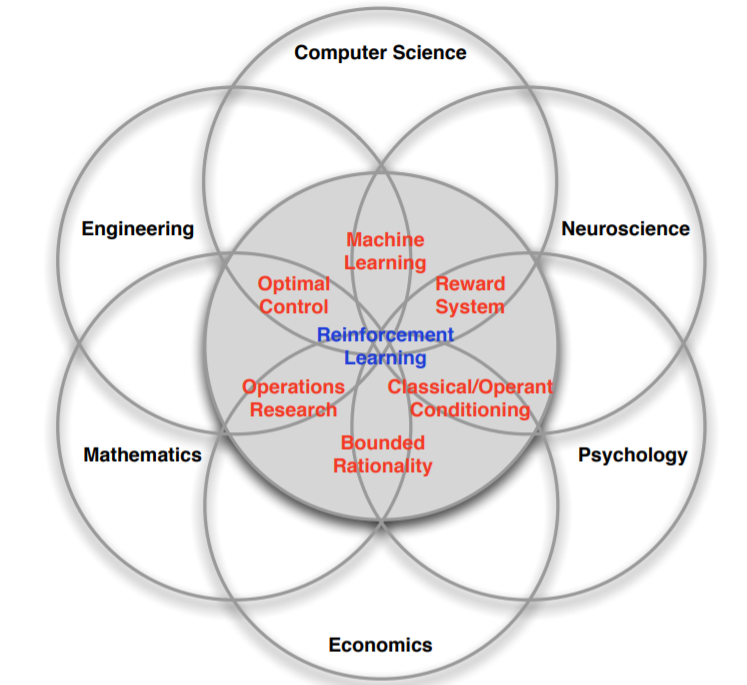
\includegraphics[width=9cm, height=8cm]{many_faces_of_RL.PNG}
\end{frame}

\begin{frame}
\frametitle{Vague (but in-vogue) Classification of Machine Learning}
\includegraphics[width=9cm, height=8cm]{MLBranches.PNG}
\end{frame}

\begin{frame}
\frametitle{Overview of the Course}
\pause
\begin{itemize}[<+->]
\item Theory of Markov Decision Processes (MDPs)
\item Dynamic Programming (DP) Algorithms
\item Reinforcement Learning (RL) Algorithms
\item Plenty of Python implementations of models and algorithms
\item Apply these algorithms to 3 Financial/Trading problems:
\begin{itemize}
\item (Dynamic) Asset-Allocation to maximize Utility of Consumption
\item Optimal Exercise/Stopping of Path-dependent American Options
\item Optimal Trade Order Execution (managing Price Impact)
\end{itemize}
\item By treating each of the problems as MDPs (i.e., Stochastic Control)
\item We will go over classical/analytical solutions to these problems
\item Then introduce real-world considerations, and tackle with RL (or DP)
\end{itemize}
\end{frame}

\begin{frame}
\frametitle{Optimal Asset Allocation to Maximize Consumption Utility}
\pause
\begin{itemize}[<+->]
\item You can invest in (allocate wealth to) a collection of assets
\item Investment horizon is a fixed length of time
\item Each risky asset has an unknown distribution of returns
\item Transaction Costs \& Constraints on trading hours/quantities/shorting
\item Allowed to consume a fraction of your wealth at specific times
\item Dynamic Decision: Time-Sequenced Allocation \& Consumption
\item To maximize horizon-aggregated Utility of Consumption
\item Utility function represents degree of risk-aversion
\item So, we effectively maximize aggregate Risk-Adjusted Consumption
\end{itemize}
\end{frame}



\begin{frame}
\frametitle{MDP for Optimal Asset Allocation problem}
\pause
\begin{itemize}[<+->]
\item {\em State} is [Current Time, Current Holdings, Current Prices]
\item {\em Action} is [Allocation Quantities, Consumption Quantity]
\item {\em Action}s limited by various real-world trading constraints
\item {\em Reward} is Utility of Consumption less Transaction Costs
\item {\em State}-transitions governed by risky asset movements
\end{itemize}
\end{frame}

\begin{frame}
\frametitle{Optimal Exercise of Path-dependent American Options}
\pause
\begin{itemize}[<+->]
\item An American option can be exercised anytime before option maturity
\item Key decision at any time is to exercise or continue
\item The default algorithm is Backward Induction on a tree/grid
\item But it doesn't work for path-dependent options 
\item Also, it's not feasible when state dimension is large
\item Industry-Standard: Longstaff-Schwartz's simulation-based algorithm
\item RL is an attractive alternative to Longstaff-Schwartz
\item RL is straightforward once Optimal Exercise is modeled as an MDP
\end{itemize}
\end{frame}

\begin{frame}
\frametitle{MDP for Optimal Options Exercise}
\pause
\begin{itemize}[<+->]
\item {\em State} is [Current Time, History of Underlying Security Prices]
\item {\em Action} is Boolean: Exercise (i.e., Payoff and Stop) or Continue
\item {\em Reward} always 0, except upon Exercise ($=$ Payoff)
\item {\em State}-transitions governed by Underlying Prices' Stochastic Process
\item Optimal Policy $\Rightarrow$ Optimal Stopping $\Rightarrow$ Option Price
\item Can be generalized to other Optimal Stopping problems
\end{itemize}
\end{frame}

\begin{frame}
\frametitle{Optimal Trade Order Execution (controlling Price Impact)}
\pause
\begin{itemize}[<+->]
\item You are tasked with selling a large qty of a (relatively less-liquid) stock
\item You have a fixed horizon over which to complete the sale
\item Goal is to maximize aggregate sales proceeds over horizon
\item If you sell too fast, {\em Price Impact} will result in poor sales proceeds
\item If you sell too slow, you risk running out of time
\item We need to model temporary and permanent {\em Price Impact}s
\item Objective should incorporate penalty for variance of sales proceeds
\item Which is equivalent to maximizing aggregate Utility of sales proceeds 
\end{itemize}
\end{frame}

\begin{frame}
\frametitle{MDP for Optimal Trade Order Execution}
\pause
\begin{itemize}[<+->]
\item {\em State} is [Time Remaining, Stock Remaining to be Sold, Market Info]
\item {\em Action} is Quantity of Stock to Sell at current time
\item {\em Reward} is Utility of Sales Proceeds (i.e., Variance-adjusted-Proceeds)
\item {\em Reward} \& {\em State}-transitions governed by {\em Price Impact Model}
\item Real-world {\em Model} can be quite complex (Order Book Dynamics)
\end{itemize}
\end{frame}


\begin{frame}
\frametitle{Week by Week (Tentative) Schedule}
\pause
\begin{itemize}[<+->]
\item W1: Markov Decision Processes \& Overview of Finance Problems
\item W2: Bellman Equations \& Dynamic Programming Algorithms
\item W3: Optimal Asset Allocation problem
\item W4: Optimal Exercise of American Options problem
\item W5: Optimal Trade Order Execution problem, and Mid-Term Exam
\item W6: Model-free Prediction (RL for Value Function Estimation)
\item W7: Model-Free Control (RL for Optimal Value Function/Policy)
\item W8: RL with Function Approximation (including Deep RL)
\item W9: Batch Methods (DQN, LSTDQ/LSPI), and Gradient TD
\item W10: Policy Gradient Algorithms
\item W11: Final Exam
\end{itemize}
\end{frame}

\begin{frame}
\frametitle{Sneak Peek into a few lectures in this course}
\begin{itemize}
\item \href{https://github.com/coverdrive/technical-documents/blob/master/finance/cme241/MertonPortfolio.pdf}{\underline{\textcolor{blue}{HJB Equation and Merton's Portfolio Problem}}}
\item \href{https://github.com/coverdrive/technical-documents/blob/master/finance/cme241/PolicyGradient.pdf}{\underline{\textcolor{blue}{Policy Gradient Theorem and Compatible Approximation Theorem}}}
\item \href{https://github.com/coverdrive/technical-documents/blob/master/finance/cme241/ValueFunctionGeometry.pdf}{\underline{\textcolor{blue}{Value Function Geometry and Gradient TD}}}
\end{itemize}
\end{frame}

\begin{frame}
\frametitle{Landmark Papers we will cover in detail}
\begin{itemize}
\item \href{https://www.jstor.org/stable/1926560}{\underline{\textcolor{blue}{Merton's solution for Optimal Portfolio Allocation/Consumption}}}
\item \href{https://people.math.ethz.ch/~hjfurrer/teaching/LongstaffSchwartzAmericanOptionsLeastSquareMonteCarlo.pdf}{\underline{\textcolor{blue}{Longstaff-Schwartz Algorithm for Pricing American Options}}}
\item \href{http://alo.mit.edu/wp-content/uploads/2015/06/Optimal-Control-of-Execution-Costs.pdf}{\underline{\textcolor{blue}{Bertsimas-Lo paper on Optimal Execution Cost}}}
\item \href{https://pdfs.semanticscholar.org/3d2d/773983c5201b58586af463f045befae5bbf2.pdf}{\underline{\textcolor{blue}{Almgren-Chriss paper on Optimal Risk-Adjusted Execution Cost}}}
\item \href{https://www.cs.toronto.edu/~vmnih/docs/dqn.pdf}{\underline{\textcolor{blue}{Original DQN paper}}} and \href{https://storage.googleapis.com/deepmind-media/dqn/DQNNaturePaper.pdf}{\underline{\textcolor{blue}{Nature DQN paper}}}
\item \href{http://www.jmlr.org/papers/volume4/lagoudakis03a/lagoudakis03a.pdf}{\underline{\textcolor{blue}{Lagoudakis-Parr paper on Least Squares Policy Iteration}}}
\item \href{http://papers.nips.cc/paper/1713-policy-gradient-methods-for-reinforcement-learning-with-function-approximation.pdf}{\underline{\textcolor{blue}{Sutton et al's paper on Policy Gradient}}}
\end{itemize}
\end{frame}


\begin{frame}
\frametitle{Similar Courses offered at Stanford}
\begin{itemize}
\item AA 228/CS 238 (Mykel Kochenderfer - Autumn 2018)
\item CS 234 (Emma Brunskill - Winter 2019)
\item MS\&E 251 (Edison Tse - Spring 2019)
\item CS 332 (Emma Brunskill - Autumn 2018)
\item MS\&E 338 (Ben Van Roy - Spring 2019)
\item MS\&E 348 (Gerd Infanger - Winter 2020)
\item MS\&E 351 (Ben Van Roy - Winter 2019)
\end{itemize}
\end{frame}

\end{document}